\chapter{Laser Interferometers for Gravitational-wave Detection}

We show in this chapter how a laser interferometer can detect
gravitational wave strain, and we present the basic design principles
of the LIGO detectors. We motivate the desire for higher laser power,
and introduce some of the details of the interferometer that are
relevant for later chapters. To reduce clutter, I do not specify the
polarization of the gravitational wave strain and use simply $h$ for
its symbol.


\section{Measuring Gravitational-wave Strain with Light}
Considering a simple Michelson interferometer consisting of a laser, a
beam splitter, and two end mirrors each a distance $L$ from the beam
splitter, one can understand intuitively why an interferometer can
detect gravitational waves. If an appropriately polarized
gravitational wave is present, it will stretch one arm and compress
the other. For two wave packets leaving the beam splitter at the same
time, each heading down a different arm, the roundtrip travel time for
the light traveling down the stretched arm is longer than that for the
light traveling down the compressed arm. For the stretched arm the
roundtrip travel time is:
\begin{equation}
t_{\mathrm{stretched}} = \frac{2 L}{c} \left( 1 + \frac{h}{2} \right),
\label{eq:trt+} 
\end{equation}
and for the compressed arm the roundtrip travel time is:
\begin{equation}
t_{\mathrm{compressed}} = \frac{2 L}{c} \left( 1 - \frac{h}{2} \right).
\label{eq:trt-} 
\end{equation}
A stationary clock at the beam splitter could, in principle, measure
the non-zero difference in arrival times, $\Delta t = 2Lh/c$, of the
two different wave packets.\footnote{It should be noted that $h$ is
  treated as a constant in Eqs. \ref{eq:trt+} and \ref{eq:trt-}. We
  use the approximation that the gravitational wave wavelength
  $\lambda_{gw}$ is much larger than the Michelson arm length
  $L$. This means that the temporal variation of $h(t)$ is negligible
  during the time it takes the photon to make its roundtrip.}

However, in practice, instead of individual wave packets, we send a
continuous electromagnetic wave into the interferometer. The
difference in travel times turns into a difference in phase:
\begin{equation}
\Delta \phi_{\mathrm{MICH}} = \omega \Delta t = \frac{2 L}{c} \omega h,
\label{eq:deltaphi}
\end{equation}
where $\omega$ is the angular frequency of the laser light. We now
introduce the modified Michelson interferometer used in LIGO, and in
this context continue the discussion of strain measurement and
sensitivity.

% reference to treatment as a wave, gauge-independent quantity.



\section{Power-recycled Fabry-P\'{e}rot Michelson Interferometers} 
The LIGO detector configuration is a power-recycled Fabry-P\'{e}rot
Michelson laser interferometer as depicted in
Fig.~\ref{fig:IFOschematic}. A beam splitter (BS) directs 1064~nm
light from a diode-pumped, power amplified, and intensity and
frequency stabilized Nd:YAG laser to the Fabry-P\'{e}rot arms, which are
made of an input test mass mirror (ITM) and an end test mass mirror
(ETM). Both arms are of length $L$ and are set to maintain nearly
perfectly destructive interference of the recombined light at the
anti-symmetric (AS) port, where a photodetector is placed to measure
any change in power. A power recycling mirror (RM) at the symmetric
port directs the constructively-interfered light back into the
interferometer.

\begin{figure}
\begin{centering}
\includegraphics{figures/IFOsimple_thesis.pdf}
\caption[Power-recycled Fabry-P\'{e}rot Michelson laser
interferometer]{Power-recycled Fabry-P\'{e}rot Michelson laser
  interferometer.}
\label{fig:IFOschematic}
\end{centering}
\end{figure}

The Fabry-P\'{e}rot arms are a modification to the Michelson that
increases the change in phase measured at the AS port compared to that
for a simple Michelson. Rather than make a single roundtrip down each
arm, the light is trapped by the Fabry-P\'{e}rot cavity, experiencing many
roundtrips before returning to the beam splitter and interfering with
the light from the other arm. The effect is that Eq.~\ref{eq:deltaphi}
for the Fabry-P\'{e}rot Michelson includes a frequency-dependent phase
gain factor, $g_{\phi}(f)$:
\begin{equation}
\Delta \phi = \frac{2 L}{c} \omega g_{\phi}(f) \Delta h.
\label{eq:deltaphi}
\end{equation}
For Enhanced LIGO, $g_{\phi} = 137$ at DC and falls off as $1/f$ after
85~Hz due to the cavity pole.


\subsection{DC readout}
\label{sec:DCreadout}
The gravitational wave readout in Enhanced LIGO did not operate
precisely at the dark fringe at the AS port. Instead, it used a small
offset from the quadratic minimum so that small changes in phase are
linear with power as is depicted in Figure~\ref{fig:DCreadout}. The
offset used was $\phi_0 \approx 6 \times 10^{-5}$~rad and the
technique is a form of homodyne detection called DC readout
\cite{Fricke2011DC}.

With a DC offset, the electric field at the AS port is $E_{AS} =
E_{BS}\sin{(\phi_0 + \Delta\phi)}$. Squaring the electric field and
expanding about $\phi_0$, we determine the power recorded by the
photodetector, $P_{AS}$:
\begin{align}
P_{AS} &= P_{BS} \sin^2{(\phi_0 + \Delta\phi)} \\
% &\approx P_{BS}\sin^2{(\phi_0)} + 2P_{BS}\sin{(\phi_0)}\cos{(\phi_0)}\Delta\phi
 &\approx P_{BS}\sin^2{(\phi_0)} + 2P_{BS}\phi_0\Delta\phi
\end{align}
The first term on the right hand side of the expanded $P_{AS}$ is the
DC power due to the static offset from the fringe. The second term on
the right hand side describes how a change in phase at the beam
splitter is converted to a change in power:
\begin{equation}
\frac{d P_{AS}}{d \phi_{BS}} =2 P_{BS} \phi_0 
%\mathrm{phase\ optical\ gain} = \frac{4 L}{c} P_{BS} \phi_0 \omega \phi_g(f) h.
\label{eq:dP_dphi}
\end{equation}
This relationship is linear and proportional to the power at the beam
splitter. Throughout this dissertation, when we refer to signals
falling in a \emph{linear regime}, we mean that they are small enough
to be well modeled by a tangent to the actual response, just as for
the case described here regarding small phase signals.

\begin{figure}
\begin{centering}
\includegraphics{figures/DCreadout.pdf}
\caption[The DC readout dark fringe]{The DC readout dark fringe. The
  AS port is not kept at the dark fringe, but is slightly offset by
  $\phi_0$. Changes in phase at the beam splitter are a linear
  function of power.}
\label{fig:DCreadout}
\end{centering}
\end{figure}



\subsection{DARM}
The most important term in LIGO is DARM, the differential arm length. This
is the length degree of freedom affected by gravitational waves. It is
defined as
\begin{equation}
\mathrm{DARM} := L_- := L_x - L_y
\end{equation}
where $L_x$ and $L_y$ are the lengths of the $x$-arm and $y$-arm,
respectively. When there is no gravitational wave, $L_-=0$, but in the
presence of a gravitational wave, the DARM signal is:
\begin{equation}
L_- = Lh
\label{eq:DARMandh}
\end{equation}
We see that $L$ is the conversion factor between GW strain and DARM.



\subsection{DARM Optical Gain}
The DARM optical gain tells how displacement is converted to power at
the AS port and has units of Watts per meter. Combining
Eqs.~\ref{eq:deltaphi}, \ref{eq:dP_dphi}, and \ref{eq:DARMandh}, the
DARM optical gain of the LIGO interferometer with DC readout is:
\begin{equation}
\frac{d P_{AS}}{dL_-} = \frac{4}{c} P_{BS} \phi_0 \omega g_{\phi}.
\label{eq:opticalgain}
\end{equation}




\section{Signal Versus Noise} 
As we see from Eq.~\ref{eq:opticalgain}, there are three fundamental
ways to increase the DARM optical gain and therefore produce more
power at the AS port for a given GW strain. The three ways are to:
\begin{enumerate}
\item make the arms longer \vspace{-10 pt}
\item increase the power at the BS \vspace{-10 pt}
\item increase the phase gain of the Fabry-P\'{e}rot arms
\end{enumerate}
However, the sensitivity of DC readout to gravitational wave strain is
dependent not only on the optical gain, but on the detector noises
that conspire to mimic gravitational waves. No matter how large a
signal one might have, it won't be found confidently, or at all, if
there is too much noise. Therefore, an increase in optical gain must
be considered in the context of the signal to noise ratio (SNR).

\subsection{Noises}
For GW detection, the signal is changing power at the AS port, and the
noises are best grouped into two categories:
\begin{enumerate}
\item displacement noise \vspace{-10 pt}
\item sensing noise
\end{enumerate}
Displacement noises affect the length of the arms and therefore create
signal at the AS port, and sensing noises affect the measurement of
the signal. 

The primary displacement noise that plagues laser interferometers is
ground motion, which physically displaces the mirrors. Another
displacement noise is thermal noise. The Brownian motion of the atoms
of the mirror displace the mirror with a fluctuating force,
\begin{equation}
F(f) = \sqrt{4k_BTb(f)},
\end{equation}
where $k_B$ is Boltzmann's constant, $T$ is temperature, and $b$ is
the mirror's dissipation.

The primary sensing noise is shot noise, a quantum mechanical effect
that creates an uncertainty in the arrival rate of photons at the
photodetector. Shot noise creates a fluctuating power with power
spectral density:
\begin{equation}
P_{SN} = \sqrt{2 P h_p \nu}
\label{eq:shotnoise}
\end{equation}
where $P$ is the DC power on the photodiode, $h_p$ is Planck's
constant, and $\nu$ is the frequency of the incident light. Shot noise
is spectrally white.

% (with units of W/$\sqrt{\mathrm{Hz}}$) 
\subsection{Noise Floor}
The detector's noise floor is limited by seismic noise below 40~Hz and
by shot noise above 200~Hz. The goal is to push the noise floor down
so that any underlying GW signals will be revealed. Whether
displacement noise or sensing noise-limited, the noise floor,
calibrated in strain, can be lowered by increasing the length of the
arms. The arm length converts strain into displacement
(Eq.~\ref{eq:DARMandh}) and the greater the effective displacement due
to GWs the better. Further improvements require considering the noise
sources individually.

\subsubsection{Displacement noise floor} 
As long as the noise floor is limited by displacement noise,
increasing the DARM optical gain does not help. The mirror
displacements, whether due to gravitational waves or due to ground
motion, are converted into power at the AS port in the exact same
way. Besides increasing the arm length, one way to improve the
displacement-limited noise floor is to simply isolate the mirrors from
the ground as best as possible.

\subsubsection{Sensing noise floor}
The sensing noise-limited sensitivity is improved by increasing the
optical gain because the more power at the AS port from GWs, the
greater the signal to sensing noise ratio. The shot-noise-limited
sensitivity is the shot noise divided by the optical gain,
\begin{equation}
h_{shot} = \sqrt{\frac{h_p}{2 P_{BS} \nu}} \frac{c}{4 \pi L g_{\phi}},
\label{eq:SNL}
\end{equation}
and has units of strain per $\sqrt{\mathrm{Hz}}$.

Here we see that the shot-noise dominated region of the noise floor
drops with increases in the optical gain. Improvement can come from
increasing the Fabry-P\'{e}rot arm phase gain or from increasing the
power at the beam splitter.  Improvement with power increases comes
about because the optical gain increases more quickly ( $\propto
P_{BS}$, see Eq.~\ref{eq:opticalgain}) than the shot noise amplitude
(which goes like $\sqrt{P_{BS}}$, assuming the DARM offset is held
constant).

Increasing the power at the beam splitter and therefore lowering the
noise floor above 200~Hz is the goal of this work. The power at the BS
is dependent on several quantities:
\begin{itemize}
\item input power \vspace{-10 pt}
\item input efficiency \vspace{-10 pt}
\item power reycling gain
\end{itemize}
Improving the Input Optics allows for greater input power and better
input efficiency. Improving the Angular Sensing and Control allows for
greater input power and better power recycling gain.



% \section{DC readout / more laser power}
% Increasing the laser power in the interferometer is a 

% Shot noise is a Poissonian process: the average number of photons
% striking a detector, $\left<x\right>$, is equal to the variance of the
% mean number of photons, $\left<x^2\right> - \left<x\right>^2$, from a
% given chunk of time $\tau$ to another. For large $\left<x\right>$, the
% distribution becomes Gaussian, but the mean and variance are still
% equivalent. Based on this property and Parseval's theorem, the power
% on a detector due to shot noise is:


%A summary of the noise budget is shown in Fig. \ref{fig:NB}.

% \begin{figure}
% \begin{centering}
% %\includegraphics[width=0.8\textwidth]{figures/.pdf}
% \caption[LIGO noise budget]{Noise budget place holder.}
% \label{fig:NB}
% \end{centering}
% \end{figure}




\section{Controlling the Interferometer}
The ability of the interferometer to provide a DARM signal to the
photodetector at the AS port depends on the many interferometer
cavities being locked, or held on resonance, all at once. The motion
of the mirrors without any control is too large for a locked state to
naturally occur. The rms pendular displacement of the mirrors without
control is 1 \micron, equivalent to a full laser wavelength. The arm
length swings from one free spectral range (FSR) to the next, never
staying put long enough at any particular FSR for light to
resonate.

The motion of the interferometer mirrors must therefore be controlled
so that resonance is achieved and so that the residual DARM motion is
small enough that the phase change it produces at the AS port can
indeed be well modeled by the linearized optical gain presented in
Eq.~\ref{eq:opticalgain}. 

% Since the strain sensitivity is determined
% by mathematically undoing the (carefully measured) effect of the
% control system on DARM, control does not directly improve the strain
% sensitivity. The purpose length control does serves is to make the
% strain measurement possible. For other degrees of freedom, such as
% angular motion, only the controlled residual matters ..  Control,
% however, introduces noise so there is a fine balance that must be
% found between too much and too little control.

% Design considerations for the control loops include how much motion at
% what frequencies can be tolerated, and the signal to noise ratio of
% the motion sensor.


% \subsection{RF Sidebands}
% Phase modulation multiplies carrier light with field
% $E_0e^{i\omega t}$ by $e^{i \Gamma \sin{(\Omega t)}}$, where $\Gamma$
% is the modulation index and $\Omega$ is the frequency of the phase
% modulation. Using the Jacobi-Anger expression,
% \begin{equation}
% e^{i z \sin{\theta}} = \sum_{n=-\infty}^{\infty} J_n(z) e^{i n \theta},
% \end{equation}
% where $J_n$ are the Bessel functions, we can write the first few terms
% (n = 0, 1, -1) of the phase-modulated field:
% \begin{equation}
% E_{modulated} = E_0 J_0(\Gamma) e^{i\omega t} + E_0 J_1(\Gamma)
% e^{i(\omega + \Omega) t} + E_0 J_{-1}(\Gamma)
% e^{i(\omega - \Omega) t} + ...
% \end{equation}
% We see that both an upper and lower primary sideband are created, with
% frequencies $\omega + \Omega$ and $\omega - \Omega$. Phase modulation
% does produce an infinite number of sidebands, yet the amplitude of the
% Bessel function decays rapidly with higher $|n|$, so only this first
% set of sidebands are significant.




\subsection{Digital Control in LIGO}
Although the interferometer is an analog instrument, it is interfaced
through a digital control system. The analog sensor signals are sent
through an analog-to-digital converter (ADC), digitally filtered, and
then sent through a digital-to-analog converter (DAC) before returning
to the interferometer's actuators as control signals. The use of a
digital control system means complex filters can be more easily
implemented than they would with analog electronics. The LSC is
acquired at 16384~Hz and the ASC at 2048~Hz. Select data is recorded
to disk.

% There are a select few control systems that remain completely analog, like
% the laser intensity stabilization servo (ISS). When the frequencies of
% interest extend beyond several tens of thousands of Hz, the use of
% computers becomes impractical.




\subsection{Mirror Suspension and Actuation}
\label{sec:suspension}
The primary interferometer optics are suspended in vacuum so that they
act like free masses at the frequencies in the GW detection band, and
so that they are isolated from ground motion. Each mirror is hung from
a single wire that loops around the bottom of the barrel of the mirror
as shown in Fig.~\ref{fig:suspension}. Stand-offs glued just above the
mirror's center of mass on both sides of the barrel mark the final
point of contact of the wire with the mirror, and both ends of the
wire are clamped to the top of a suspension cage.

\begin{figure}
\begin{centering}
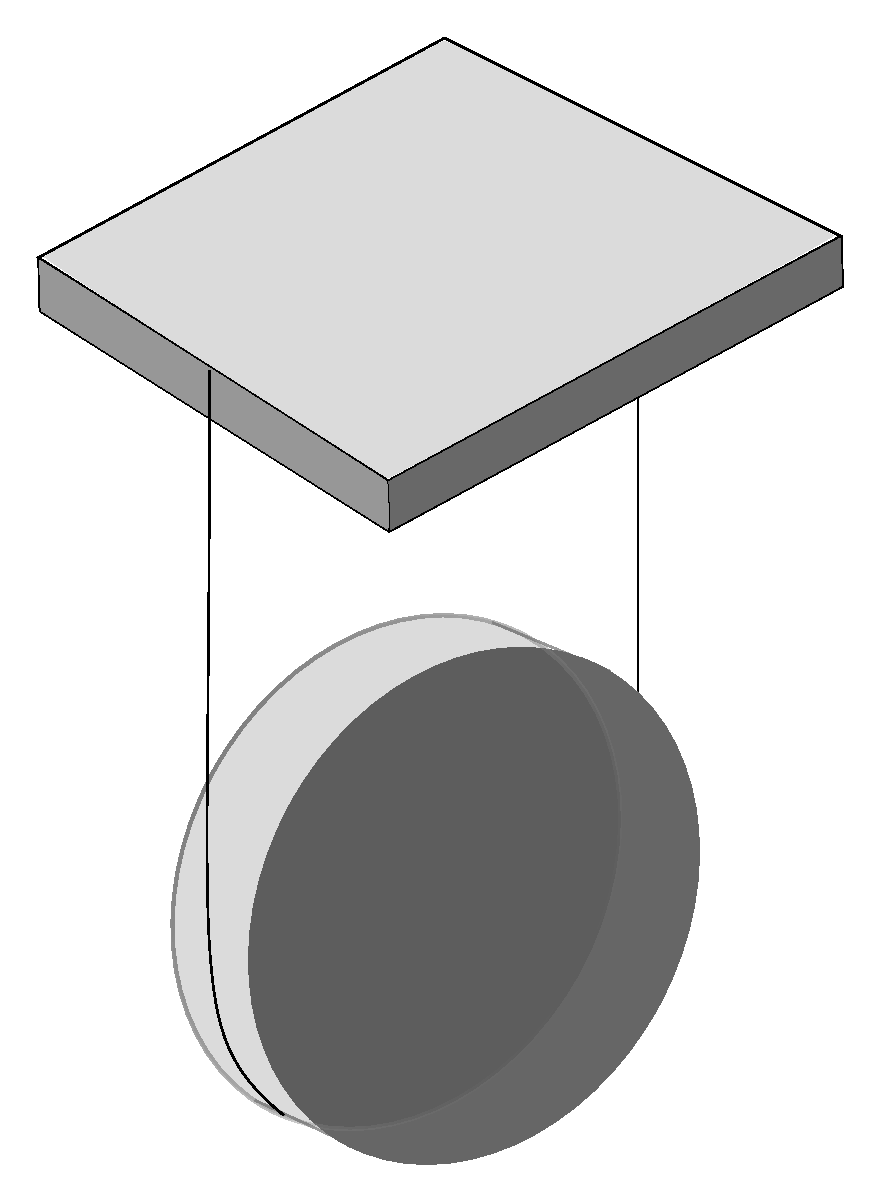
\includegraphics[width=0.3\textwidth]{/Users/kate/kate-thesis/figures/suspension.pdf}
\caption[Sketch of a LIGO suspension]{Sketch of a LIGO suspension.}
\label{fig:suspension}
\end{centering}
\end{figure}

Each mirror is equipped with four optical sensor and electro-magnetic
(OSEM) actuators for providing control to the mirror. Magnets arranged
to form the four corners of a square are glued on the mirror's back
surface, and the OSEM units envelop them. Length control of the
cavities, for instance, sends current of the same magnitude through
each coil on a given mirror to provide a piston force for changing the
mirror's position.

Minimal contact with the mirrors is necessary to avoid thermal
noise. Therefore, the suspensions provide minimal damping to the
mirrors. Damping for the large optics is instead achieved
electronically through the use of optical levers.\footnote{The OSEMs
  also provide local velocity damping, although the angular OSEM
  feedback is turned off when the interferometer is locked.} The
optical levers provide velocity damping only (no DC control) between
0.2~Hz and 2~Hz. The open loop transfer function of the optical lever
servo is in Appendix~\ref{sec:oplevOLG}.

% The suspensions are AC damped at all times for each of the large
% optics through optical lever witnesses. Keeping the mirrors quiet
% enough with respect to their local ground is necessary to allow for
% the initial locking of the interferometer, so each suspended optic,
% small and large, is quieted by its OSEM signals during the initial
% locking stages. After the interferometer is locked, the angular OSEM
% feedback is turned off, and the position OSEM feedback remains.
